\chapter{Labview}
\lineaLateral

\begin{resumenCapitulo}
Este capítulo describe el diseño e implementación de la Interfaz Hombre-Máquina (HMI) y la arquitectura de software desarrollada para la gestión integral del brazo robótico Mitsubishi Movemaster EX. Se detalla la transición de un sistema de control tradicional hacia una infraestructura moderna basada en el patrón de diseño \textbf{Productor-Consumidor}, que permite la ejecución paralela de tareas críticas como la adquisición de telemetría a alta velocidad, el procesamiento de protocolos binarios inspirados en Modbus y la automatización de trayectorias mediante archivos externos. 
El enfoque principal es demostrar cómo la integración de LabVIEW con el firmware del microcontrolador permite un control determinista, una visualización robusta de variables físicas y un entorno de operación escalable.
\end{resumenCapitulo}


\section{Interfaz de Usuario en LabVIEW}
La estación de control fue desarrollada en LabVIEW, aprovechando su capacidad para la gestión de datos mediante una arquitectura de manejador de mensajes encolados (QMH). La interfaz se organiza en un panel principal con una barra de navegación lateral que permite conmutar entre tres pestañas operativas: \textbf{Dashboard}, \textbf{Control Manual} y \textbf{Control PID}.

\subsection{Panel de Monitoreo (Dashboard)}
La pestaña de \textit{Dashboard} funciona como el centro de diagnóstico principal. En esta vista se presentan indicadores visuales de tipo carátula para cada una de las articulaciones (Cadera, Hombro, Codo, Antebrazo y Muñeca). Para cada eje, el sistema despliega en tiempo real:
\begin{itemize}
	\item \textbf{Conteo de Pasos:} Valor absoluto del encoder tras el procesamiento en el microcontrolador.
	\item \textbf{Velocidad:} Cálculo derivado de la variación de pasos por unidad de tiempo.
	\item \textbf{Estado de Alarmas:} Indicadores de seguridad para los finales de carrera y estados de error.
\end{itemize}

\begin{figure}[h]
	\centering
	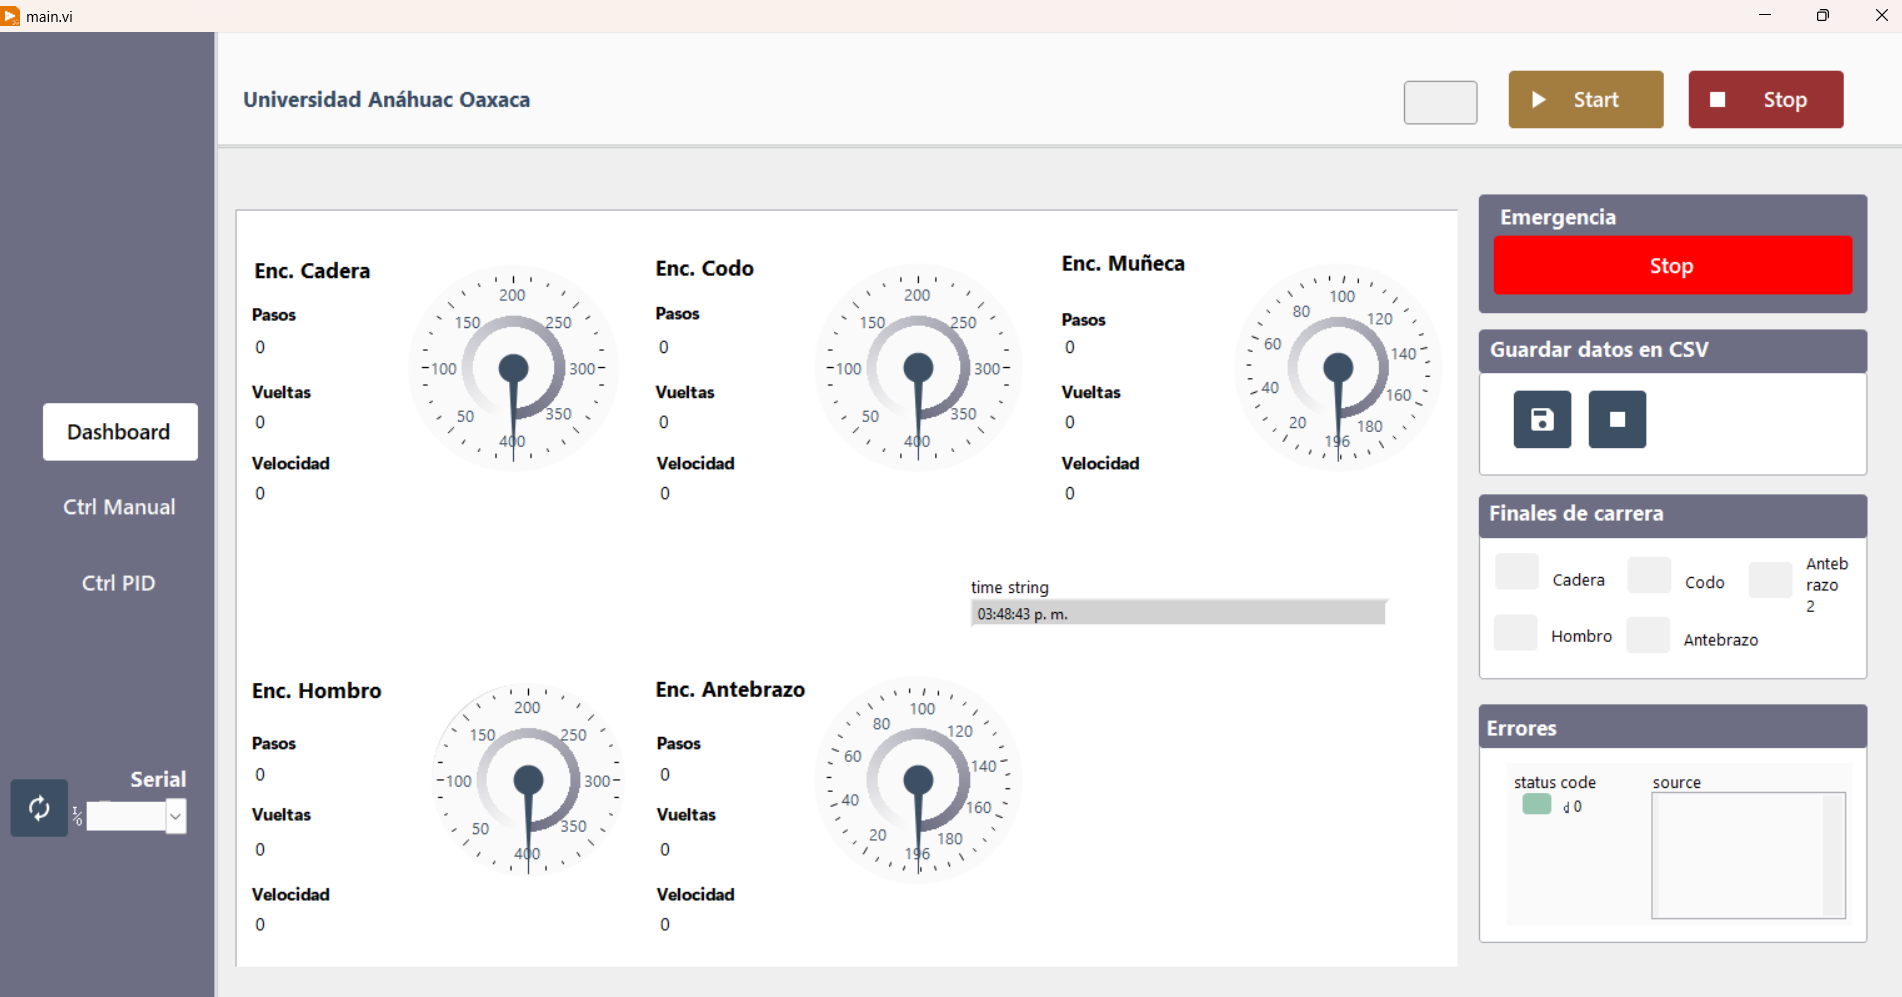
\includegraphics[width=1\linewidth]{images/Interfaz/dashboard}
	\caption[Dashboard.]{Ventana de lectura de los encoders.}
	\label{fig:dashboard}
\end{figure}


\subsection{Modos de Control: Manual y Trayectorias}
La pestaña de \textbf{Control Manual} ofrece al operario dos métodos para manipular el brazo:
\begin{enumerate}
	\item \textbf{Control por PWM:} Ajuste directo del ciclo de trabajo para cada motor mediante controles deslizantes (\textit{sliders}), permitiendo movimientos finos para el posicionamiento inicial del robot.
	\item \textbf{Rutina desde Archivo:} Funcionalidad avanzada que permite cargar un archivo externo (CSV o Excel) con trayectorias predefinidas. El sistema lee estas coordenadas y las envía de forma secuencial al controlador para su ejecución automática.
\end{enumerate}

\begin{figure}[h]
	\centering
	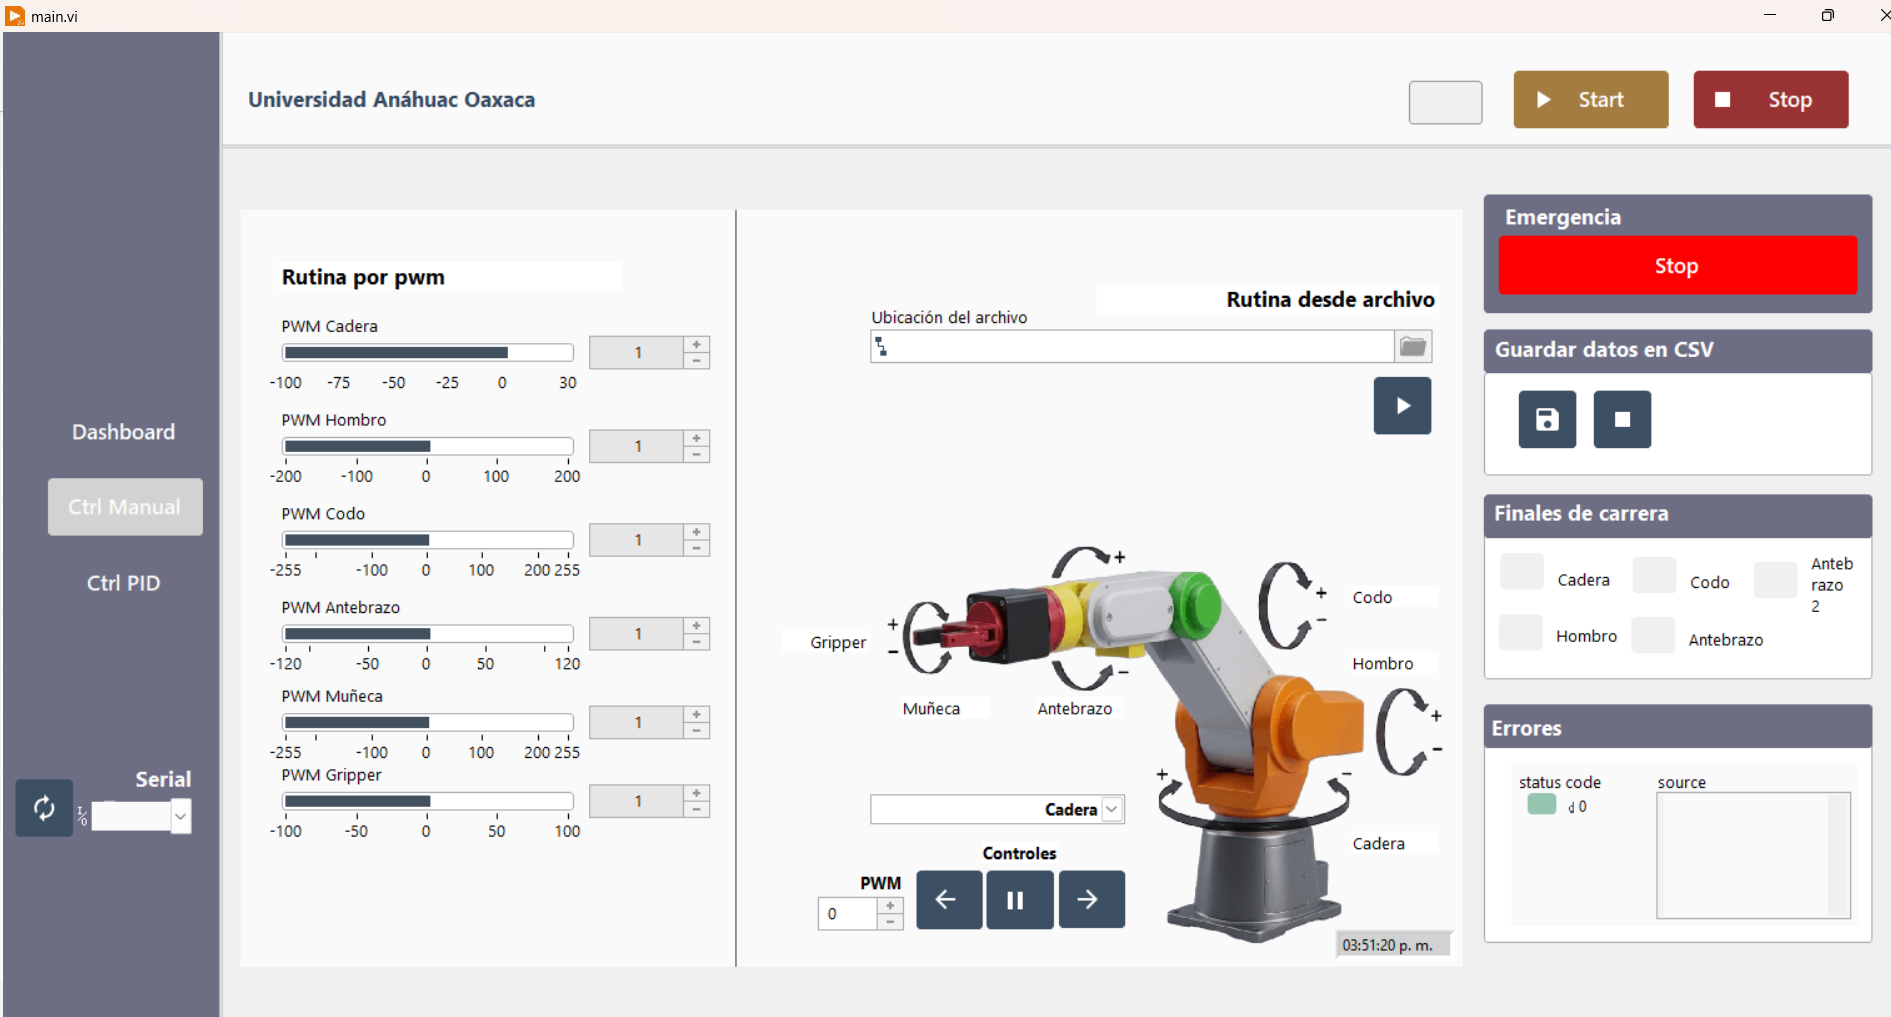
\includegraphics[width=1\linewidth]{images/Interfaz/control}
	\caption{Ventana de control de la interfaz.}
	\label{fig:control}
\end{figure}



\subsection{Sintonización y Control PID}
La pestaña de \textbf{Control PID} está diseñada para la optimización dinámica del movimiento. Esta sección permite al usuario ajustar las constantes de control ($K_p$, $T_i$, $T_d$) de manera individual para cada articulación. Incluye una gráfica de tiempo real (\textit{Waveform Chart}) que superpone el \textbf{Setpoint} (posición deseada) frente a la \textbf{Posición Actual}, permitiendo visualizar el error, el sobreimpulso y el tiempo de asentamiento del sistema bajo diferentes condiciones de carga.

\begin{center}
	\fcolorbox{green!30!black}{green!5}{
		\begin{minipage}{1\textwidth}
			\textbf{Nota de Seguridad:} Independientemente de la pestaña activa, la interfaz mantiene un botón de \textbf{Paro de Emergencia} global que, al activarse, envía una señal prioritaria para frenar todos los motores y bloquear las articulaciones.
		\end{minipage}
	}
\end{center}

\begin{figure}[h]
	\centering
	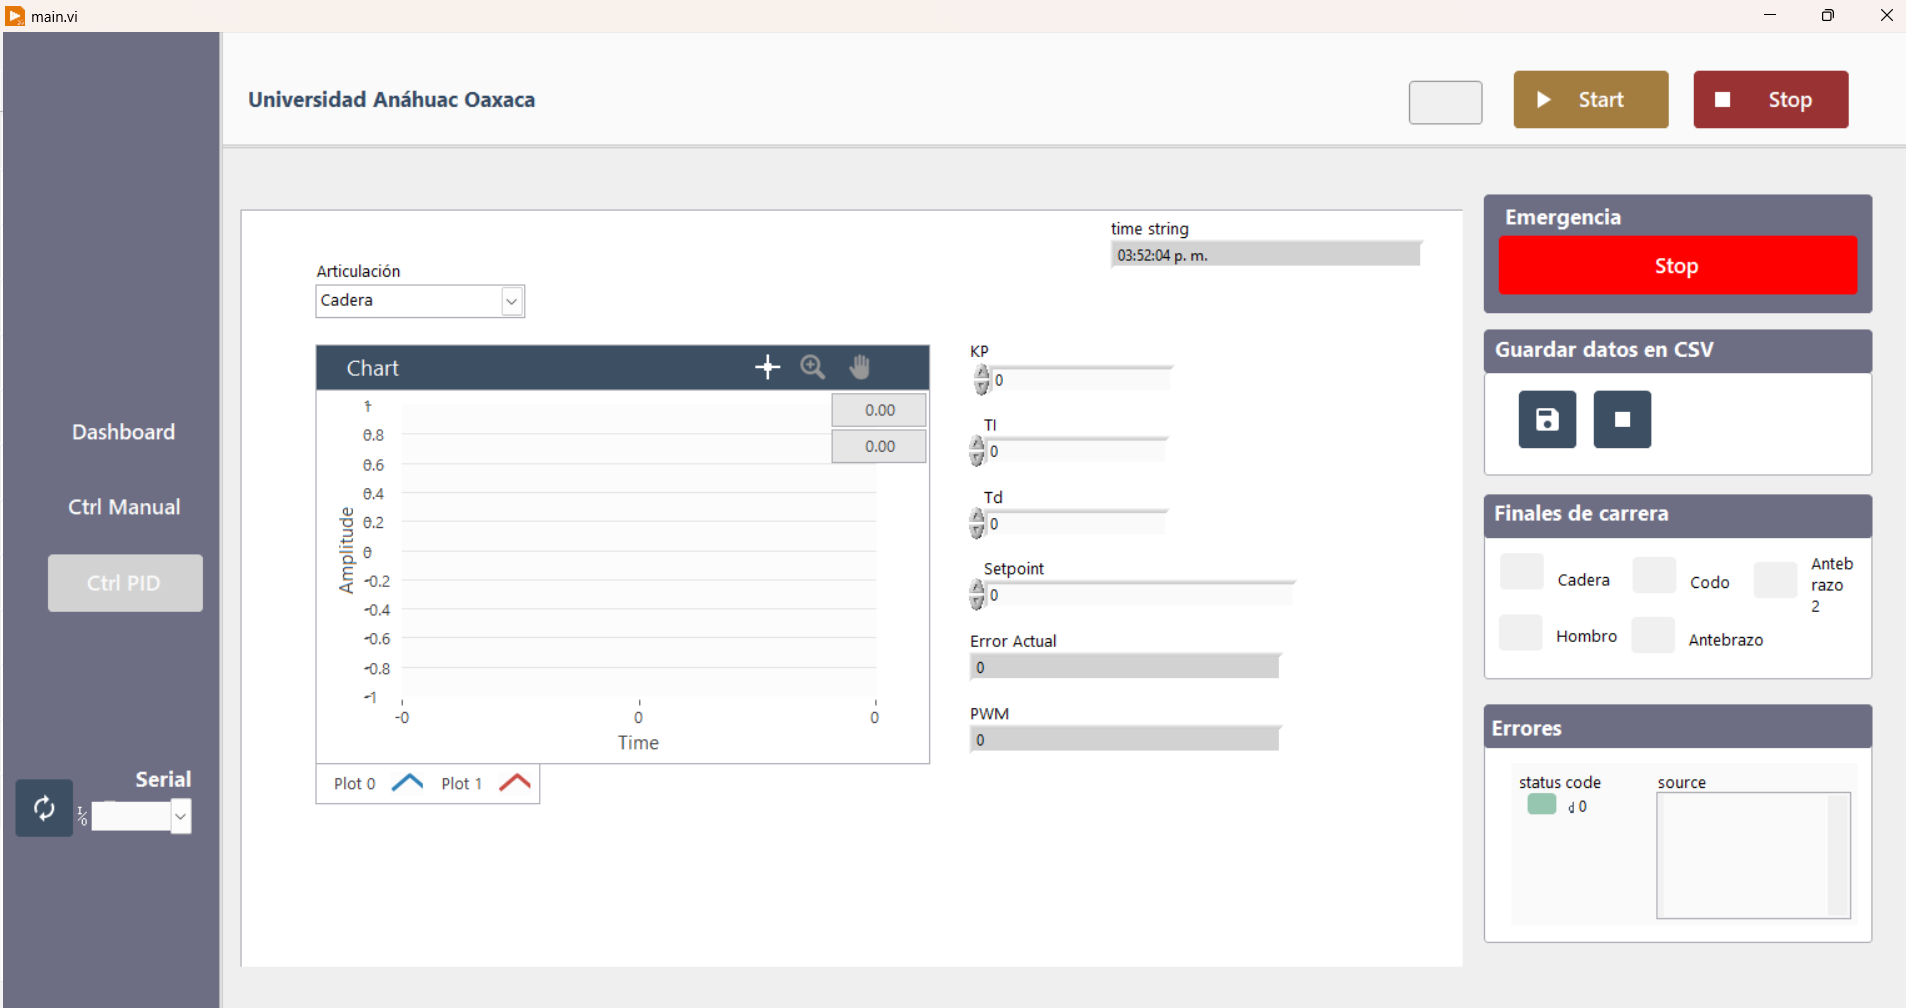
\includegraphics[width=1\linewidth]{images/Interfaz/pid}
	\caption{Ventana de PID de la interfaz.}
	\label{fig:pid}
\end{figure}

\section{Arquitectura del programa}


\subsection{Bucle Productor: Gestión de Eventos de la UI}
El núcleo de la interacción con el usuario reside en un bucle principal que implementa una \textbf{Estructura de Eventos}. Este loop actúa como el \textbf{Productor} del sistema, donde cada control del panel frontal (botones, interruptores y menús) tiene asignada una lógica específica. Ante cualquier interacción, el bucle genera indicaciones que son distribuidas a los subprocesos correspondientes, asegurando que la interfaz no se bloquee durante operaciones de cálculo intensivo.

\begin{figure}[h]
	\centering
	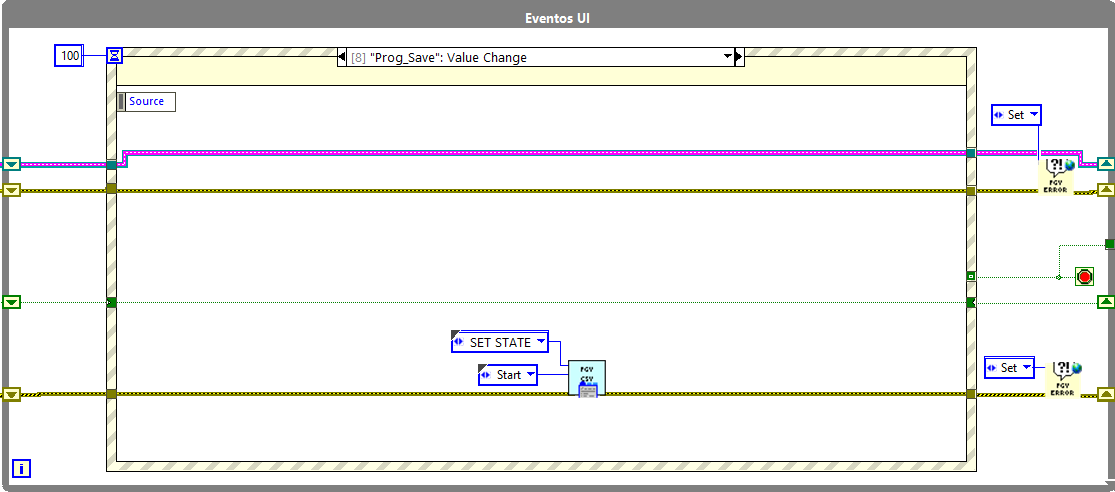
\includegraphics[width=0.7\linewidth]{images/Interfaz/eventosUI}
	\caption{Bucle de Eventos UI.}
	\label{fig:eventosui}
\end{figure}

\begin{figure}[h]
	\centering
	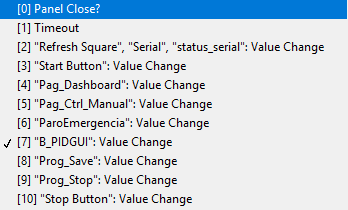
\includegraphics[width=0.4\linewidth]{images/Interfaz/eventos}
	\caption{Para cada botón de la interfaz principal, existe un evento.}
	\label{fig:eventos}
\end{figure}

\begin{figure}[h]
	\centering
	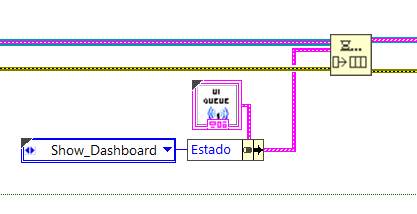
\includegraphics[width=0.7\linewidth]{images/Interfaz/uiqueue}
	\caption{La \textbf{ UI Queue} es el tipo de dato que se comparte entre el \textbf{ loop de Eventos UI y el loop de procesamiento de la UI.} }
	\label{fig:uiqueue}
\end{figure}

\begin{figure}[h]
	\centering
	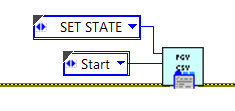
\includegraphics[width=0.7\linewidth]{images/Interfaz/comunicacionConDataLogger}
	\caption{Se utiliza la \textbf{FGV CSV} para que desde \textbf{el loop de Eventos UI se mande al loop de Data Logger}.}
	\label{fig:comunicacioncondatalogger}
\end{figure}

\begin{figure}[h]
	\centering
	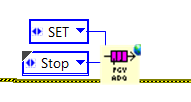
\includegraphics[width=0.7\linewidth]{images/Interfaz/comunicacionConLoopAdquisicion}
	\caption{Se utliza la \textbf{FGV de ADQ} para que desde \textbf{el loop de Eventos UI mande comandos al loop de Adquisición}}
	\label{fig:comunicacionconloopadquisicion}
\end{figure}

\begin{figure}[h]
	\centering
	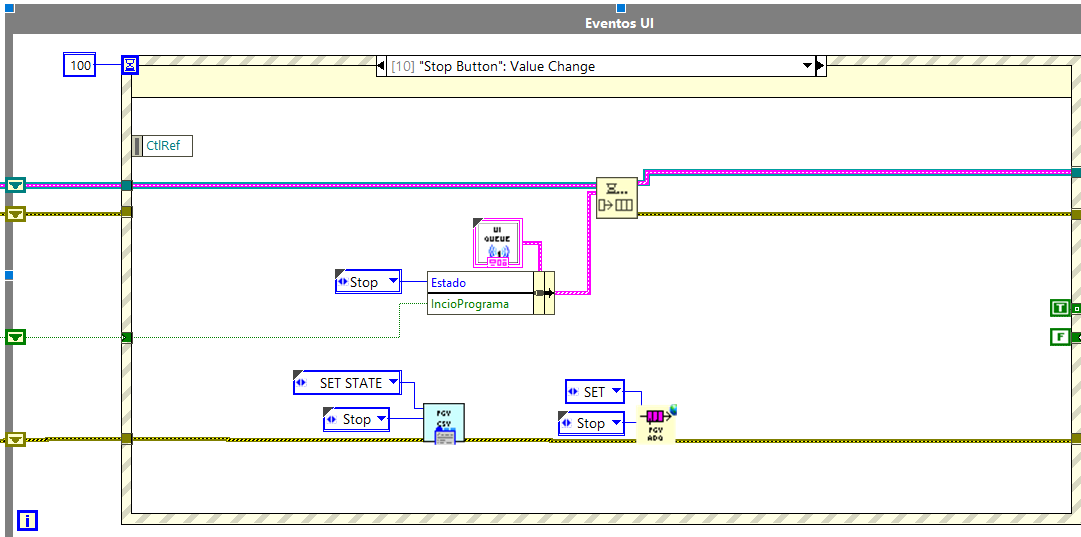
\includegraphics[width=0.7\linewidth]{images/Interfaz/casoStopEventosUI}
	\caption{El caso que ocurre al presionar stop es un ejemplo de como existe comunicación desde Eventos UI a los otros tres loops.}
	\label{fig:casostopeventosui}
\end{figure}

\clearpage

\subsection{Loop de Procesamiento y Control de Flujo}
El bucle productor se comunica directamente con el loop de procesamiento de la UI para coordinar el inicio y la detención de las rutinas de control. Esta transferencia de directivas se realiza mediante el uso de una \textbf{Cola (Queue)}, la cual permite un paso de mensajes asíncrono y ordenado, garantizando que el sistema transite entre estados operativos de manera determinista.

\begin{table}[h!]
	\centering
	\renewcommand{\arraystretch}{1.5}
	\caption{Descripción de estados y acciones del bucle de procesamiento de la UI.}
	\label{tab:casos_loop_ui}
	\begin{tabularx}{\textwidth}{|l|X|}
		\hline
		\rowcolor{green!20}
		\textbf{Caso / Estado} & \textbf{Acción Ejecutada en el Software} \\ \hline
		\textbf{PID\_GUI} & Realiza la inserción dinámica del subpanel correspondiente a la configuración y monitoreo del control PID en la interfaz principal. \\ \hline
		\textbf{Show\_Dashboard} & Carga e inserta el subpanel del Dashboard, permitiendo la visualización de la telemetría general y el estado del robot. \\ \hline
		\textbf{Show\_Control} & Gestiona la visualización del panel de control manual, habilitando los comandos directos hacia las articulaciones. \\ \hline
		\textbf{Stop} & Detiene de forma segura todos los subpaneles activos. Adicionalmente, invoca al \textit{VI Caller} para enviar una señal de parada obligatoria y finalizar los procesos en ejecución. \\ \hline
		\textbf{Idle (Default)} & Actúa como el estado de reposo activo. Se ejecuta cíclicamente cada \textbf{50 ms} para actualizar el estado de los finales de carrera y refrescar los indicadores de seguridad en la UI. \\ \hline
	\end{tabularx}
\end{table}

\begin{figure}[h]
	\centering
	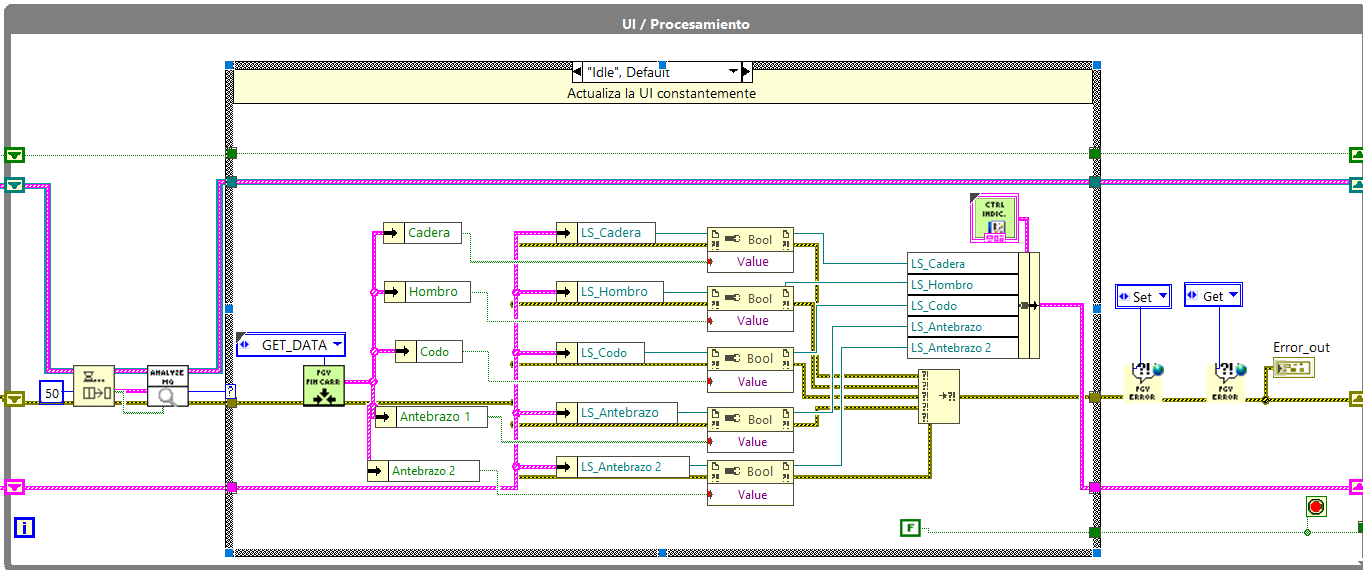
\includegraphics[width=1\linewidth]{images/Interfaz/loopprocesamiento}
	\caption{Loop donde se procesan los comandos provenientes del \textbf{loop de Eventos UI}.}
	\label{fig:loopprocesamiento}
\end{figure}

\begin{figure}
	\centering
	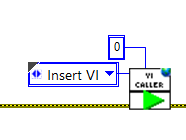
\includegraphics[width=0.7\linewidth]{images/Interfaz/vicaller}
	\caption{Este VI es el que se encarga de la lógica de insertar el subpanel. Sus únicos parámetros son el número del subpanel que se quiere insertar (0 para dashboard, 1 para control manual y 2 para lo del pid) y la acción 'Insert VI'.}
	\label{fig:vicaller}
\end{figure}

\clearpage

\subsection{Registro de Datos y Uso de Variables Globales Funcionales (FGV)}
La gestión del almacenamiento de datos en archivos de formato delimitado por comas (\textbf{.csv}) se centraliza a través de una \textbf{Variable Global Funcional (FGV)}. Esta estructura se utiliza como punto de control maestro para inicializar el registro, gestionar la escritura de las muestras y finalizar el cierre del archivo de manera segura al concluir el programa, evitando la pérdida de información o la corrupción del archivo.



\begin{figure}[h]
	\centering
	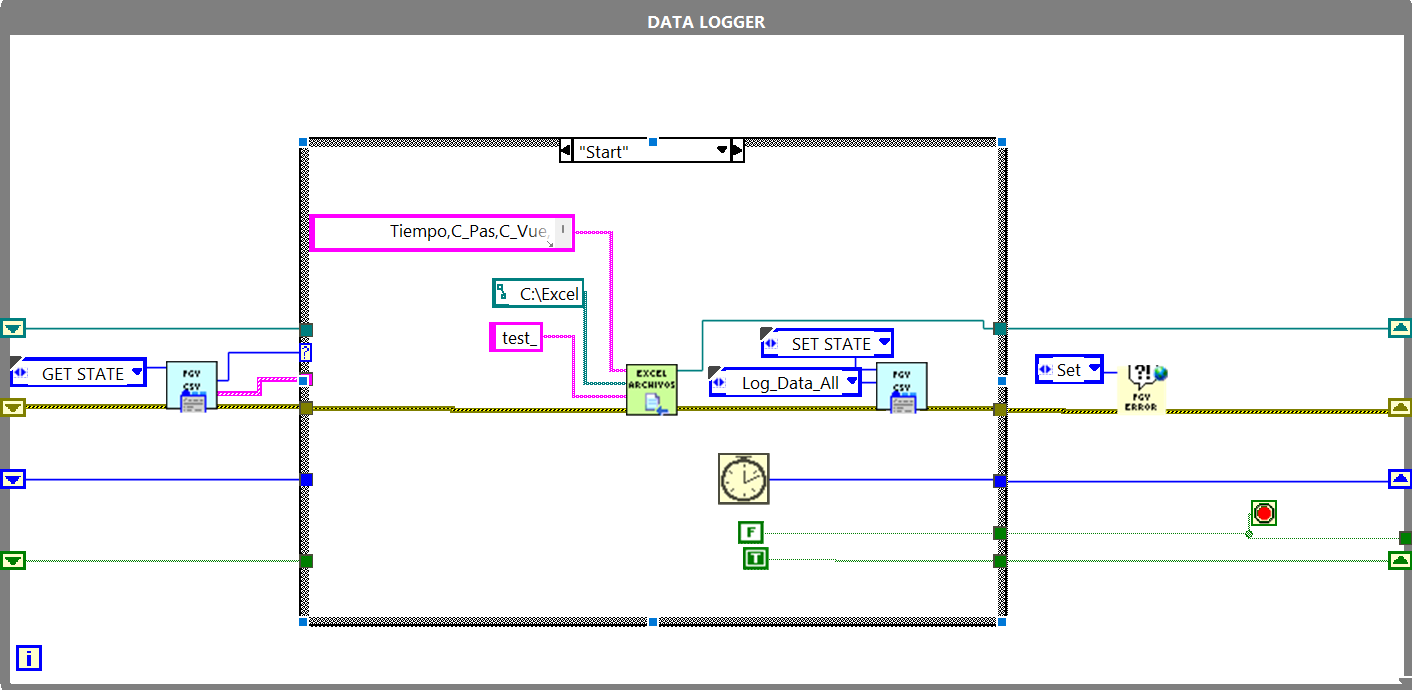
\includegraphics[width=1\linewidth]{images/Interfaz/datalogger}
	\caption{Este loop actúa según los comandos que manda la \textbf{FGV CSV} a la case structure.}
	\label{fig:datalogger}
\end{figure}

\begin{table}[h!]
	\centering
	\renewcommand{\arraystretch}{1.5}
	\caption{Flujo lógico del sistema de registro de datos en archivos CSV.}
	\label{tab:flujo_guardado_datos}
	\begin{tabularx}{\textwidth}{|l|X|}
		\hline
		\rowcolor{green!20}
		\textbf{Estado / Paso} & \textbf{Descripción de la Operación} \\ \hline
		\textbf{Start} & Inicializa el proceso de guardado. Se genera automáticamente un nuevo archivo con el prefijo \texttt{test\_}, almacenándolo en el directorio predefinido por el usuario. \\ \hline
		\textbf{Log\_Data\_All} & Fase de escritura activa. El sistema extrae los valores de telemetría (pasos, vueltas y velocidad) de todos los encoders y los concatena en el archivo CSV de forma cíclica. \\ \hline
		\textbf{Idle (Default)} & Estado de espera activa. El bucle permanece en este caso mientras no se detecte un cambio de estado en la interfaz de guardado, optimizando el uso de CPU. \\ \hline
		\textbf{Stop} & Finaliza la sesión de registro. Se cierra el flujo de escritura del archivo CSV, garantizando que todos los datos en el búfer se guarden correctamente en el disco antes de liberar el recurso. \\ \hline
	\end{tabularx}
	\begin{flushleft}
		\footnotesize \textbf{Nota:} Este ciclo de ejecución es independiente del lazo principal de la UI, permitiendo que el guardado de datos no interfiera con la fluidez de la visualización de los instrumentos.
	\end{flushleft}
\end{table}

\begin{figure}[h]
	\centering
	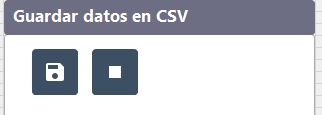
\includegraphics[width=0.7\linewidth]{images/Interfaz/botonescsv}
	\caption{Estos botones son los encargados de inicializar el loop y detenerlo.}
	\label{fig:botonescsv}
\end{figure}

\clearpage

\subsection{Loop de Adquisición de Telemetría y Gestión VISA}
Para la recepción de los datos provenientes del microcontrolador Arduino, se implementó un loop de adquisición dedicado. Este proceso se encarga de extraer y decodificar la telemetría enviada de forma constante. Como medida de seguridad y robustez, el loop de adquisición solo inicia su ejecución si existe una \textbf{Sesión de VISA activa}; en caso contrario, el proceso permanece inactivo para evitar excepciones o errores de desbordamiento de búfer. Asimismo, el bucle productor tiene la facultad de detener este proceso de forma inmediata según el estado global del sistema.

\begin{figure}[h]
	\centering
	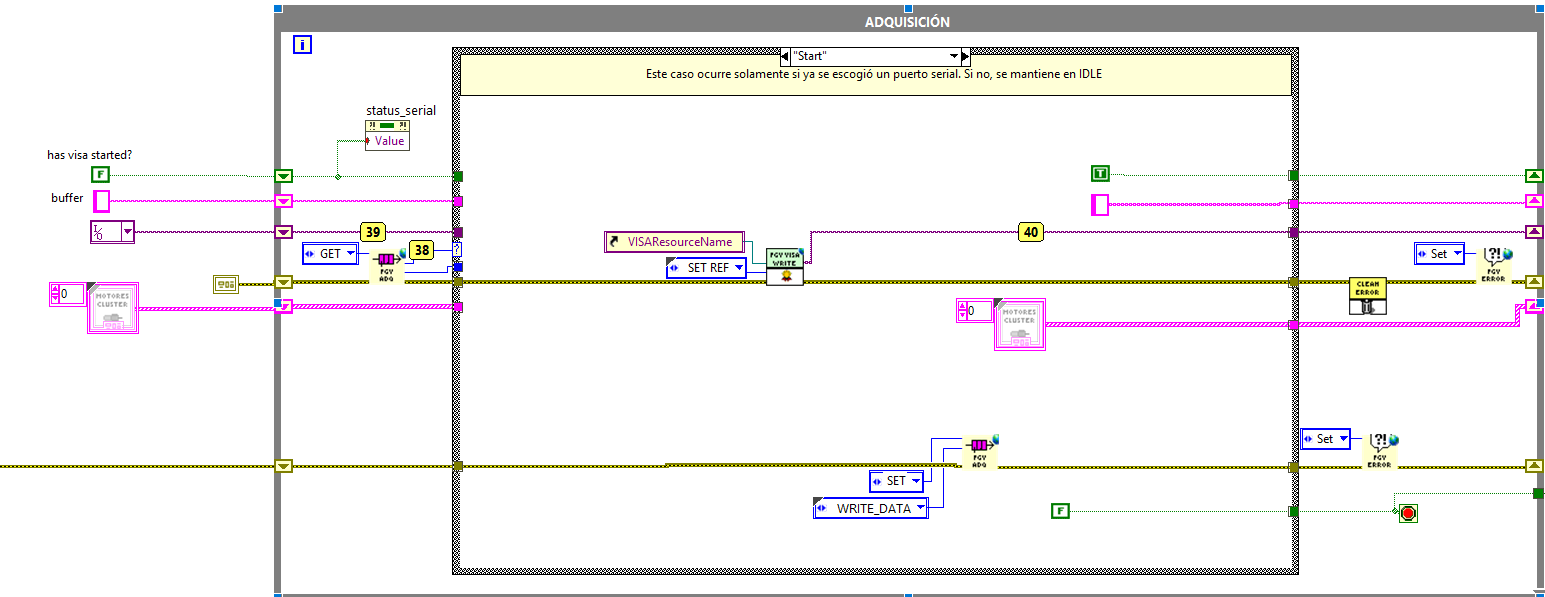
\includegraphics[width=1\linewidth]{images/Interfaz/adquisicion}
	\caption{Loop de adquisición de datos. Es controlado por la \textbf{FGV ADQ}.}
	\label{fig:adquisicion}
\end{figure}

\begin{figure}[h]
	\centering
	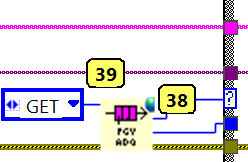
\includegraphics[width=0.7\linewidth]{images/Interfaz/fgvadq}
	\caption{La \textbf{FGV ADQ} es quien decide el comportamiento de la case structure,}
	\label{fig:fgvadq}
\end{figure}


\begin{table}[h]
	\centering
	\renewcommand{\arraystretch}{1.5}
	\caption{Lógica operativa del bucle de comunicación VISA y decodificación.}
	\label{tab:flujo_visa_comms}
	\begin{tabularx}{\textwidth}{|l|X|}
		\hline
		\rowcolor{green!20}
		\textbf{Estado} & \textbf{Descripción Técnica de la Operación} \\ \hline
		\textbf{Start} & Invoca la \textbf{FGV VISA Write} para inicializar la sesión de comunicación. En esta fase se resetean los registros internos y se realiza la transición automática al estado \textit{Write Data}. \\ \hline
		\textbf{Write Data} & Implementa una estructura condicional basada en el estado de la sesión:
		\begin{itemize}
			\item \textbf{Sesión no iniciada:} El sistema permanece en espera sin ejecutar acciones.
			\item \textbf{Sesión activa:} Llama al VI \textbf{Decode Modbus}. Los datos procesados se distribuyen en arreglos (según la configuración de \textit{Global Init}) hacia la \textbf{FGV CSV} para registro y hacia el \textbf{VI Dashboard} para la actualización del subpanel.
		\end{itemize} \\ \hline
		\textbf{Reconnect} & Ejecuta un cierre forzado de la sesión VISA actual para reestablecer la comunicación utilizando los parámetros actualizados del indicador, retornando posteriormente al estado \textit{Idle}. \\ \hline
		\textbf{Stop} & Finaliza la comunicación: cierra el recurso VISA, vacía los búferes de entrada/salida y reinicia los \textit{Shift Registers} e indicadores para asegurar un inicio limpio en la siguiente sesión. \\ \hline
		\textbf{Idle} & Estado de espera activa donde el sistema monitorea nuevas peticiones de la UI sin consumir recursos de comunicación serial. \\ \hline
	\end{tabularx}
\end{table}

\clearpage

\section{Subpanels}
\subsection{Interfaz principal}
Al iniciar la aplicación y antes de que el usuario ejecute el programa principal, la interfaz se presenta en un estado de reposo funcional. En este punto, es notable la existencia de un espacio vacío o hueco en la región central del panel frontal; este espacio corresponde al contenedor del \textbf{Subpanel}, el cual ha sido reservado específicamente para alojar de manera dinámica las distintas vistas de monitoreo y control.

A pesar de la ausencia de una vista cargada, los elementos de supervisión global y control de flujo permanecen visibles y operativos en los laterales de la ventana. Los componentes disponibles en este estado inicial se describen a continuación:

\begin{itemize}
	\item \textbf{Selectores de Vista:} Tres botones principales ubicados en la columna izquierda permiten al operario decidir qué subpanel se insertará en el área central. Por configuración predeterminada del sistema, la primera vista asignada al iniciar la comunicación es el \textbf{Dashboard}.
	\item \textbf{Control de Ejecución Maestro:} En la parte superior derecha se ubican los botones de \textbf{Start} y \textbf{Stop}, encargados de inicializar o finalizar la arquitectura de comunicación VISA y los lazos de procesamiento.
	\item \textbf{Módulo de Seguridad:} Un botón de \textbf{Paro de Emergencia} de alta visibilidad permite la interrupción inmediata de todas las señales PWM hacia los motores.
	\item \textbf{Gestión de Datos:} La sección de Guardar datos en CSV permite configurar el registro de telemetría en disco antes de iniciar el movimiento del brazo.
	\item \textbf{Monitoreo de Periféricos:} Se presentan indicadores para los \textbf{Finales de Carrera} de cada articulación y un visualizador de \textbf{Códigos de Error}, los cuales permiten diagnosticar el estado del hardware de forma previa a la operación dinámica.
\end{itemize}


\begin{figure}[h]
	\centering
	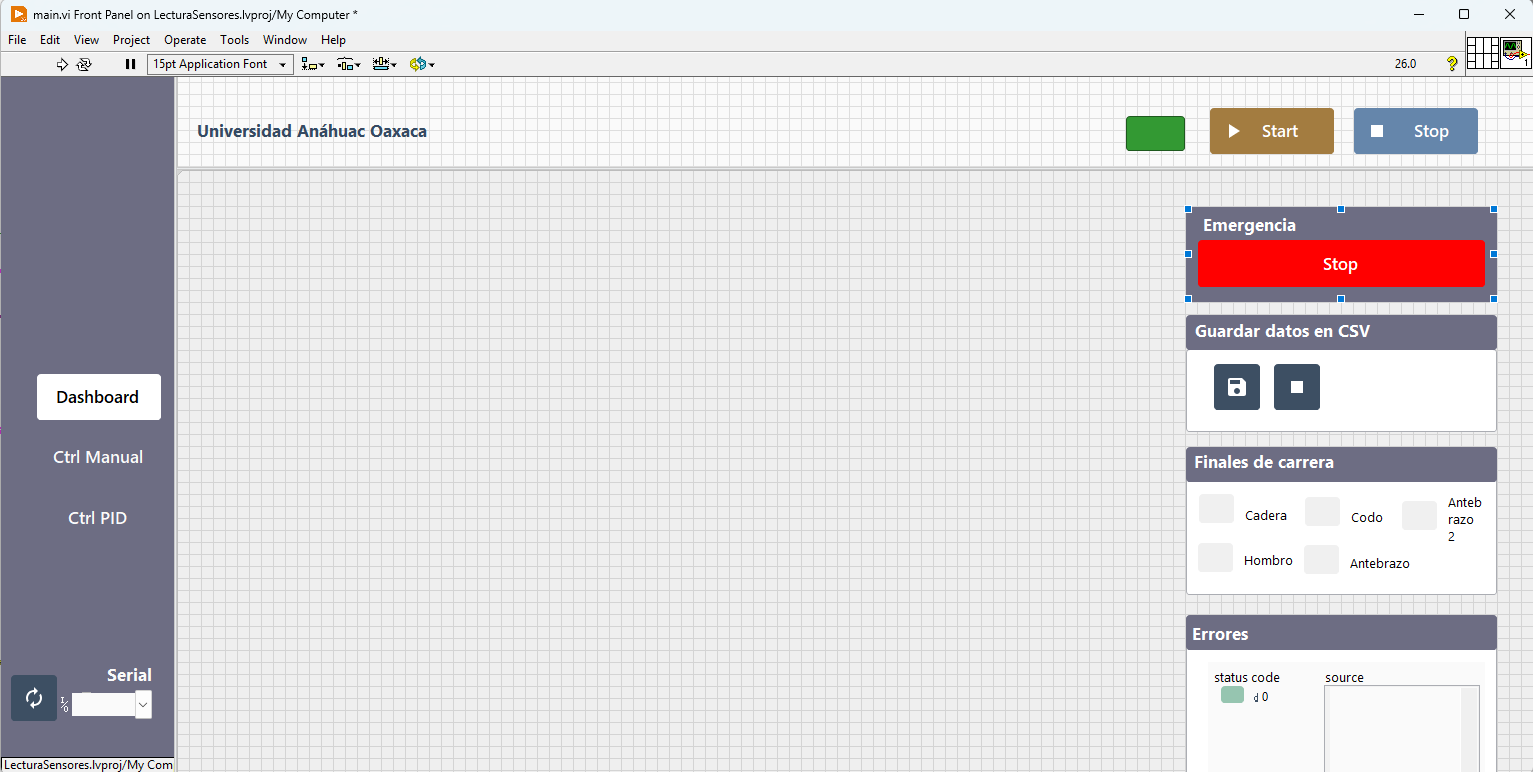
\includegraphics[width=1\linewidth]{images/Interfaz/interfazPrincipal}
	\caption{Interfaz cuando no existe ningún subpanel insertado.}
	\label{fig:interfazprincipal}
\end{figure}

\begin{figure}[h]
	\centering
	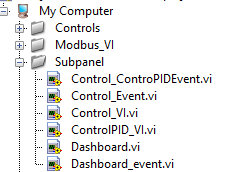
\includegraphics[width=0.7\linewidth]{images/Interfaz/carpetasubpanel}
	\caption{Carpeta donde se guardan los subpanels.}
	\label{fig:carpetasubpanel}
\end{figure}


\clearpage
\subsection{Subpanel de Dashboard}

El VI del Dashboard está diseñado para visualizar la telemetría en tiempo real sin sobrecargar el procesador, utilizando una arquitectura orientada a eventos. Su funcionamiento se basa en la recepción asíncrona de datos y la actualización selectiva de la interfaz gráfica.

\subsubsection{Gestión de Datos mediante User Events}
A diferencia de un bucle de consulta convencional (\textit{polling}), este subpanel utiliza una \textbf{Estructura de Eventos de Usuario}. El flujo de información se describe a continuación:
\begin{itemize}
	\item \textbf{Recepción de Telemetría:} El evento se dispara únicamente cuando llega un nuevo arreglo de datos desde el loop de adquisición principal. Este arreglo contiene la información procesada de los encoders de todas las articulaciones.
	\item \textbf{Actualización de Indicadores:} Una vez recibido el paquete, se invoca al VI \textbf{Refresh Ind}. Este sub-VI actúa como un motor de renderizado que mapea los valores numéricos del arreglo hacia los indicadores gráficos, barras de progreso y visualizadores de posición en el panel frontal del Dashboard.
\end{itemize}

\subsubsection{Control de Ejecución y Determinismo}
La eficiencia del Dashboard reside en su capacidad de permanecer en estado de espera hasta que existan datos nuevos que procesar, manteniendo una latencia mínima. 

Para garantizar un cierre seguro de la aplicación, el sistema monitorea el estado del canal de eventos. En el momento en que el evento de usuario es destruido o invalidado por el programa principal (al presionar el botón de \textit{Stop} o cerrar la sesión), el bucle de ejecución interno detecta esta condición y detiene el proceso de forma inmediata, liberando los recursos de memoria asignados al subpanel.

\begin{figure}[h]
	\centering
	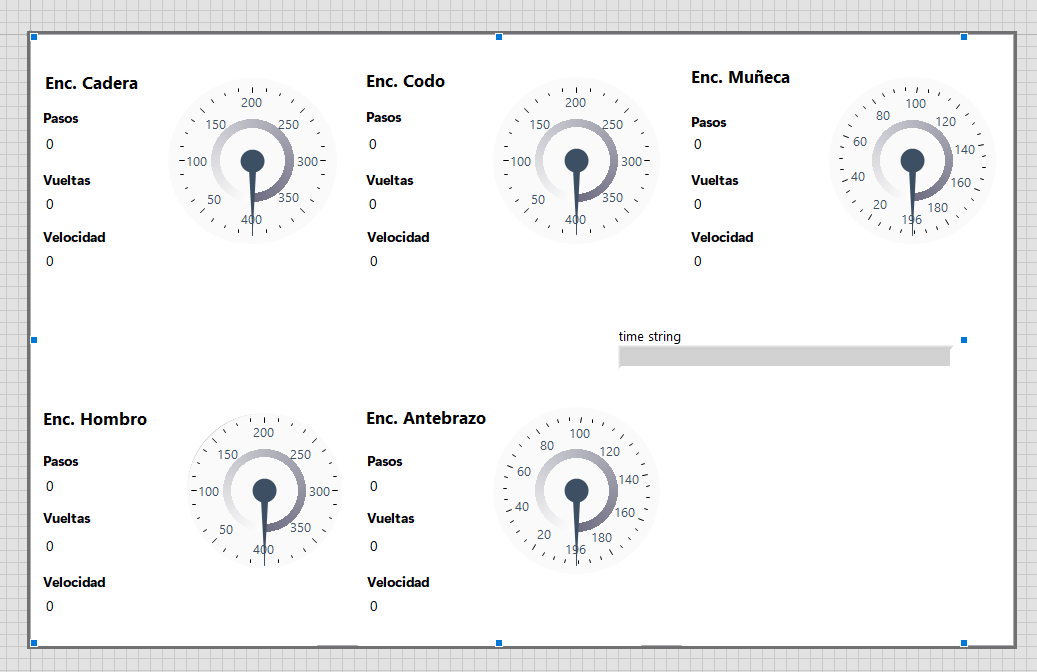
\includegraphics[width=0.7\linewidth]{images/Interfaz/subpaneldashboard}
	\caption{Front panel al abrir el \textbf{Dashboard.vi}}
	\label{fig:subpaneldashboard}
\end{figure}

\begin{figure}[h]
	\centering
	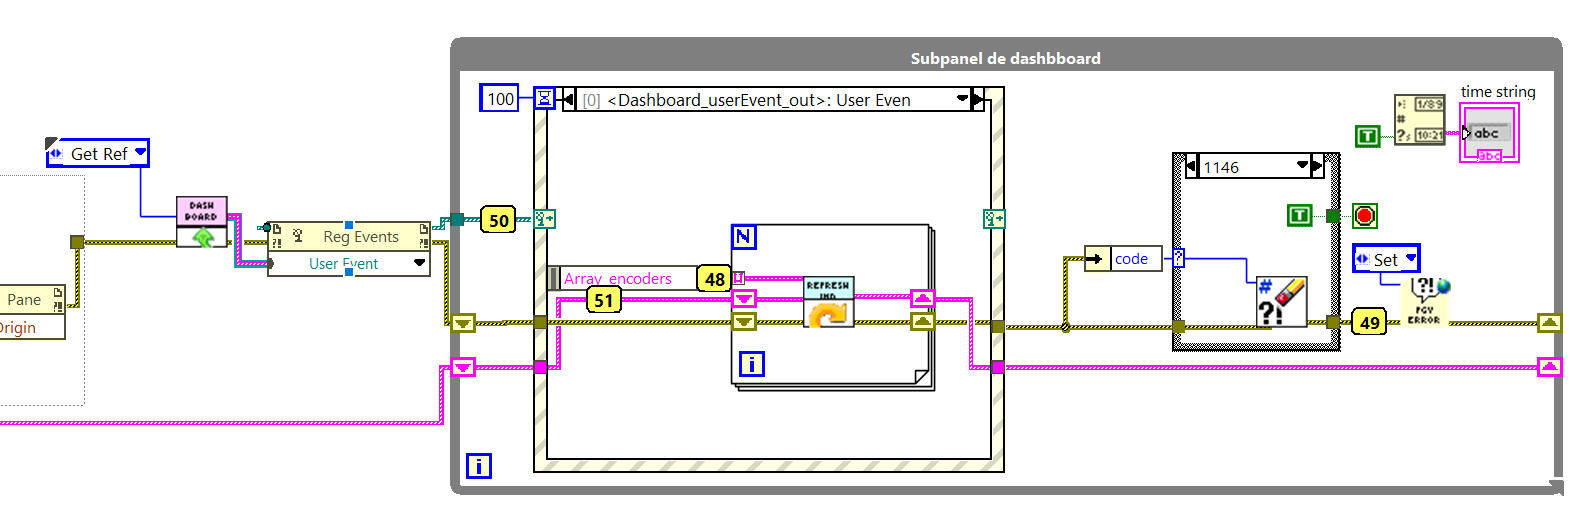
\includegraphics[width=1\linewidth]{images/Interfaz/loopdashboard}
	\caption{Único loop dentro del subpanel de dashboard.}
	\label{fig:loopdashboard}
\end{figure}

\clearpage

\section{Subpanel de Control}
El subpanel de control constituye la interfaz operativa principal para la manipulación dinámica del brazo Mitsubishi. Su diseño integra tres niveles de abstracción de movimiento, gestionados mediante una estructura de eventos que prioriza la seguridad y la precisión.

\subsubsection{Control de Movimiento Continuo (Sliders)}
Para el posicionamiento rápido de las articulaciones, se implementó un sistema de \textbf{desplazamiento continuo} mediante controles tipo \textit{slider}. 
\begin{itemize}
	\item \textbf{Lógica de Señal:} Cada articulación cuenta con un slider independiente que traduce su posición en un valor de \textbf{PWM} específico. Al desplazar el control, el sistema envía una instrucción constante al Arduino Mega.
	\item \textbf{Seguridad:} El movimiento es ininterrumpido hasta que el usuario libera el control o hasta que el firmware detecta la activación de un \textbf{final de carrera}, momento en el cual el sistema fuerza un estado de freno activo para evitar daños mecánicos.
\end{itemize}

\subsubsection{Control Discreto de Precisión (Botones de Paso)}
Ubicados en la parte inferior de la interfaz, se encuentran los botones de avance incremental. Estos controles están diseñados para tareas que requieren un ajuste fino de la posición:
\begin{itemize}
	\item \textbf{Funcionamiento:} Al ser presionados, el brazo ejecuta un avance de una cantidad de pasos predefinida (por ejemplo, 400 pasos) con el ciclo de trabajo PWM indicado en el panel. 
	\item \textbf{Utilidad:} Este modo permite al operario realizar acercamientos controlados hacia objetos o puntos de referencia sin el riesgo de inercia asociado al control continuo.
\end{itemize}

\subsubsection{Ejecución de Trayectorias Automatizadas (Módulo Excel)}
La funcionalidad más avanzada del subpanel es la ejecución de rutinas externas. Este proceso permite automatizar movimientos complejos mediante la carga de archivos de hoja de cálculo:
\begin{itemize}
	\item \textbf{Estructura de la Rutina:} El archivo de Excel contiene columnas dedicadas para cada articulación, especificando el \textbf{tiempo de ejecución} y el \textbf{valor de PWM} deseado.
	\item \textbf{Control de Flujo:} El software recorre el archivo fila por fila. Para garantizar el determinismo, el sistema utiliza un protocolo de confirmación: tras enviar una línea de comando, el subpanel entra en un estado de espera hasta recibir una señal de objetivo alcanzado por parte del microcontrolador, asegurando que la trayectoria física coincida fielmente con la programada.
\end{itemize}


\begin{figure}[h]
	\centering
	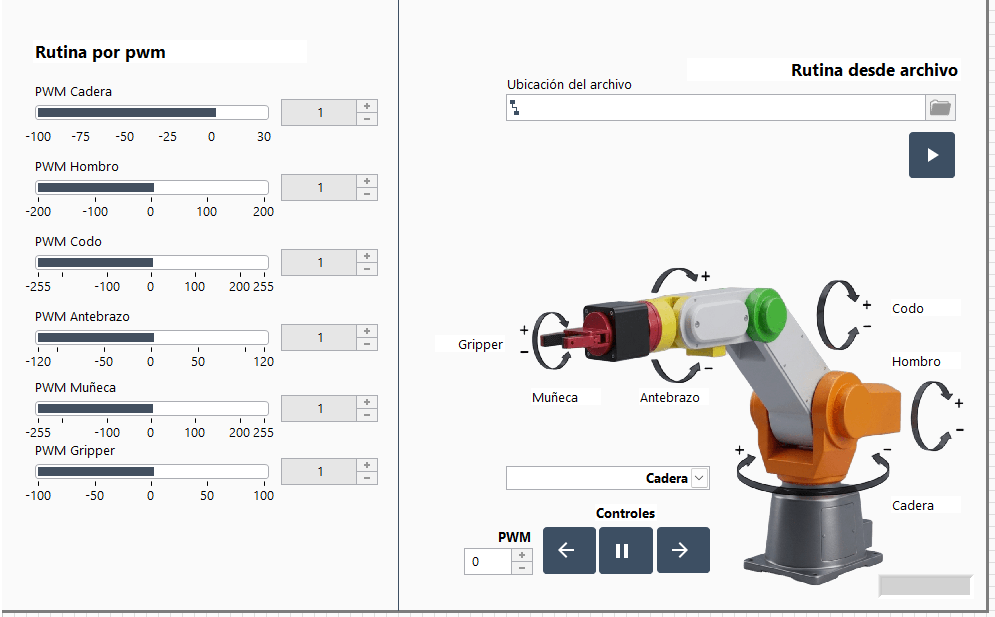
\includegraphics[width=1\linewidth]{images/Interfaz/frontpanelcontrol}
	\caption{Subpanel de controlVI.}
	\label{fig:frontpanelcontrol}
\end{figure}

\begin{figure}[h]
	\centering
	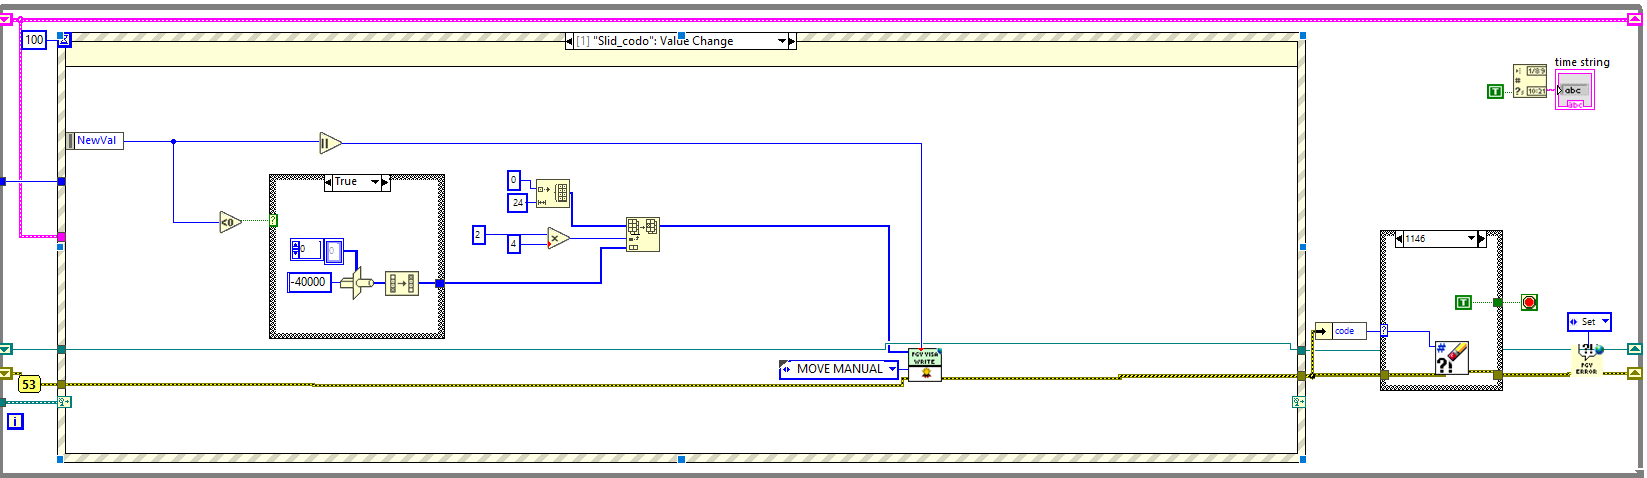
\includegraphics[width=1\linewidth]{images/Interfaz/loopcontrolvi}
	\caption{Único loop con el que funciona este subpanel.}
	\label{fig:loopcontrolvi}
\end{figure}

\begin{table}[h!]
	\centering
	\renewcommand{\arraystretch}{1.5}
	\caption{Lógica de operación del Subpanel de Control Manual y Trayectorias.}
	\label{tab:subpanel_control}
	\begin{tabularx}{\textwidth}{|l|X|}
		\hline
		\rowcolor{blue!10}
		\textbf{Evento / Control} & \textbf{Acción y Protocolo de Comunicación} \\ \hline
		\textbf{Slid\_[Articulación]} & Al detectar un cambio en el slider, se envía una instrucción al \textbf{VISA Write} para iniciar un movimiento continuo en la dirección indicada. El motor avanza hasta que el sistema detecta la activación de un \textbf{final de carrera}. \\ \hline
		\textbf{B\_izq / B\_der} & Envía un comando de movimiento discreto de \textbf{400 pasos} en el sentido seleccionado. La velocidad de este desplazamiento está determinada por el valor de PWM configurado en el indicador de la interfaz. \\ \hline
		\textbf{Pause} & Genera y transmite un \textbf{arreglo de ceros} hacia el Arduino. El firmware reconoce este paquete como una instrucción de parada inmediata para todos los actuadores. \\ \hline
		\textbf{Play File} & Ejecuta la secuencia almacenada en el archivo Excel seleccionado. La lógica realiza un recorrido \textbf{fila por fila} y luego por columnas (extrayendo PWM y tiempo por motor) para enviarlo al bloque de escritura serial. \\ \hline
		\textbf{Sincronización Excel} & El sistema implementa un control de flujo: tras enviar un comando del archivo, el subpanel entra en espera hasta recibir una \textbf{confirmación del Arduino} que indique que los motores han alcanzado la posición antes de enviar la siguiente fila. \\ \hline
	\end{tabularx}
\end{table}
\clearpage

\section{VI principales}
\subsection{FGV VISA WRITE}


En sistemas con múltiples procesos concurrentes, el acceso simultáneo a un recurso de hardware único, como un puerto serie, puede generar colisiones de datos y errores de ejecución. Para mitigar este riesgo, se desarrolló la \textbf{FGV VISA Write}. Esta estructura cumple dos funciones primordiales:

\begin{enumerate}
	\item \textbf{Control de Concurrencia:} Al encapsular la referencia de VISA dentro de un \textit{Shift Register} interno, se garantiza que solo un lazo de ejecución a la vez pueda escribir en el búfer de transmisión, evitando condiciones de carrera entre los subpaneles y el loop de procesamiento.
	\item \textbf{Estandarización de Mensajes:} Siguiendo una arquitectura inspirada en el protocolo Modbus (similar a la decodificación en el Arduino), la FGV actúa como el motor de empaquetado de información. Todos los comandos salientes se estructuran bajo un formato de trama consistente que incluye cabecera, código de función, carga útil (\textit{payload}) y una suma de verificación (CRC).
\end{enumerate}

A continuación, se detalla la lógica implementada en cada uno de los estados de la FGV para la gestión de las tramas de control:

\begin{table}[h!]
	\centering
	\renewcommand{\arraystretch}{1.5}
	\caption{Descripción de funciones y estructura de tramas en FGV VISA Write.}
	\label{tab:fgv_visa_write_cases}
	\begin{tabularx}{\textwidth}{|l|X|}
		\hline
		\rowcolor{green!20}
		\textbf{Estado / Acción} & \textbf{Estructura de la Trama y Función} \\ \hline
		\textbf{SET / GET REF} & Permite almacenar y recuperar la referencia de sesión VISA en el \textit{Shift Register}. Asegura que todos los módulos utilicen el mismo canal de comunicación abierto durante la inicialización. \\ \hline
		\textbf{SEND ROUTINE} & Diseñado para la ejecución de trayectorias desde Excel. Envía una trama con: \texttt{Header} (0X3A) | \texttt{FX=3} | \texttt{Payload=0} | \texttt{PWM (Int16)} | \texttt{Tiempo (Int16)} | \texttt{CRC}. Los datos de PWM y tiempo se extraen directamente de la fila correspondiente del archivo. \\ \hline
		\textbf{EMERGENCY STOP} & Prioriza la seguridad del sistema enviando una trama de detención inmediata: \texttt{Header (0x3A)} | \texttt{FX=1} | \texttt{Payload=0} | \texttt{Array de 0s} | \texttt{CRC}. Esta instrucción fuerza al Arduino a apagar todas las salidas PWM. \\ \hline
		\textbf{MOVE MANUAL} & Vinculado a los controles de paso discreto del subpanel. Estructura: \texttt{Header} (0X3A) | \texttt{FX=1} | \texttt{PWM} | \texttt{Dirección/Pasos ($\pm$400)} | \texttt{CRC}. Envía la dirección relativa exacta para mover la articulación seleccionada. \\ \hline
	\end{tabularx}
\end{table}

\begin{figure}[h]
	\centering
	
\includegraphics[width=0.4\linewidth]{images/Interfaz/visawriteicon}
	\caption{Icono del visa writre.}
	\label{fig:visawriteicon}
\end{figure}


\begin{figure}[h]
	\centering
	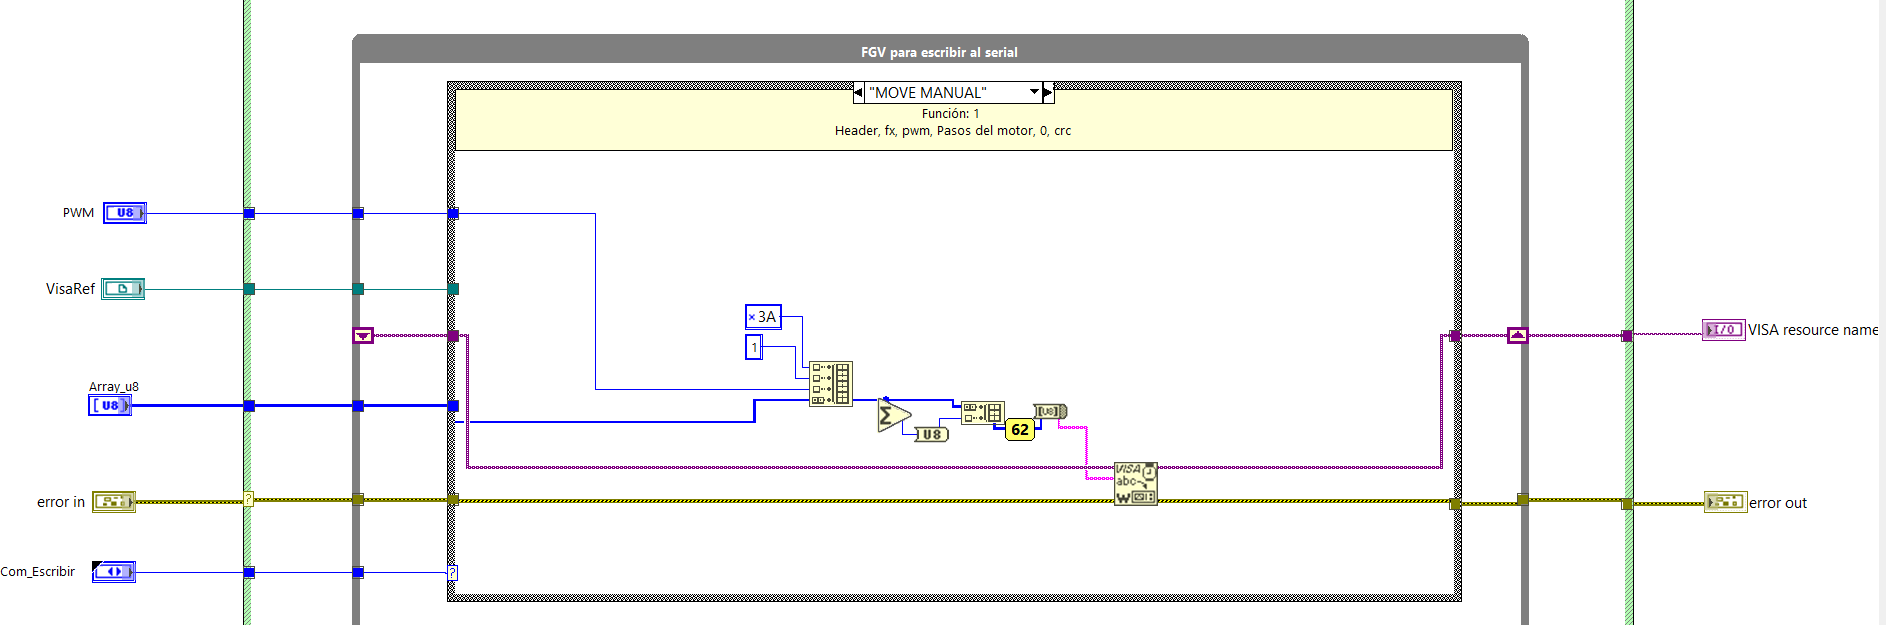
\includegraphics[width=1\linewidth]{images/Interfaz/fgvvisawrite}
	\caption{Loop del VI: VISA WRITE.}
	\label{fig:fgvvisawrite}
\end{figure}

\clearpage

\subsection{decodeModbusMessage}
\begin{figure}[h]
	\centering
	
\includegraphics[width=0.4\linewidth]{images/Interfaz/modbus}
	\caption{Icono del decodeModbusMessage.}
	\label{fig:modbus}
\end{figure}

\subsubsection{Definiciones de Estructura de Datos}

Para la correcta interpretación del flujo de información en el sistema de telemetría, se establecen las siguientes definiciones técnicas:

\begin{description}
	\item[\textbf{Trama (Datagrama):}] Representa la unidad mínima de información con sentido lógico. Corresponde a un mensaje individual de exactamente \textbf{31 bytes}, el cual encapsula la cabecera de sincronización, el estado operativo de los 6 motores, los finales de carrera, la telemetría de posición de los encoders y el byte de verificación (CRC).
	
	\item[\textbf{Lote de Datos (Buffer de Recepción):}] Se define como el conjunto masivo de bytes extraídos del puerto serial en un único ciclo de lectura. Su longitud es variable y se determina dinámicamente como el producto de la longitud de una \textit{Trama} por el número de paquetes configurados por el usuario en el módulo de inicialización global (\textit{Global Init}).
\end{description}

\subsection{Procesamiento y Decodificación de Datos: Decode Modbus Message}

Para convertir el flujo binario del puerto serial en datos legibles, se desarrolló el VI \textbf{Decode Modbus Message}. Este módulo actúa como un motor de des-serialización que procesa el segmento de datos recibido para extraer la telemetría de manera organizada.

\subsubsection{Estructura de la Lógica de Decodificación}
El funcionamiento del VI se rige por los parámetros establecidos en el bloque de inicialización global (\textit{Global Init}) y sigue un proceso iterativo descrito a continuación:

\begin{enumerate}
	\item \textbf{Verificación de Segmento:} El programa primero valida que el buffer de entrada contenga la cantidad mínima de información requerida. El tamaño esperado se calcula dinámicamente como:
	\[ \text{Tamaño Segmento} = \text{Longitud de Trama (31 bytes)} \times \text{Número de Paquetes} \]
	
	\item \textbf{Extracción Iterativa:} Mediante un bucle \textit{While}, el VI segmenta el bloque de datos para extraer una \textbf{Trama} a la vez. Este proceso asegura que, aunque lleguen múltiples actualizaciones en un solo ciclo de lectura, ninguna se pierda.
	
	\item \textbf{Des-serialización (Unflatten from String):} Cada trama es procesada por la función \textit{Unflatten from String}. Se utiliza una configuración de tipo \textbf{Little Endian} para coincidir con la arquitectura de memoria del ATMega2560. En este paso, los bytes se convierten de nuevo en sus tipos de datos originales: \texttt{uint8\_t} para estados y \texttt{int32\_t} para las posiciones de los encoders.
	
	\item \textbf{Concatenación y Distribución:} Los valores descifrados de cada motor se acumulan en arreglos al finalizar cada iteración del ciclo. Una vez que el segmento de datos ha sido analizado por completo, los arreglos finales se envían hacia las terminales de salida del VI.
\end{enumerate}

\subsubsection{Interconectividad de Datos}
La salida de este VI es el punto de origen de la información para los procesos paralelos del software. Tanto el \textbf{Subpanel de Dashboard} (para la visualización en tiempo real) como el \textbf{Loop de Registro CSV} (para el almacenamiento en disco) consumen estos arreglos de datos sincronizados, garantizando que todos los módulos trabajen con la misma base de información validada.



\begin{figure}[h]
	\centering
	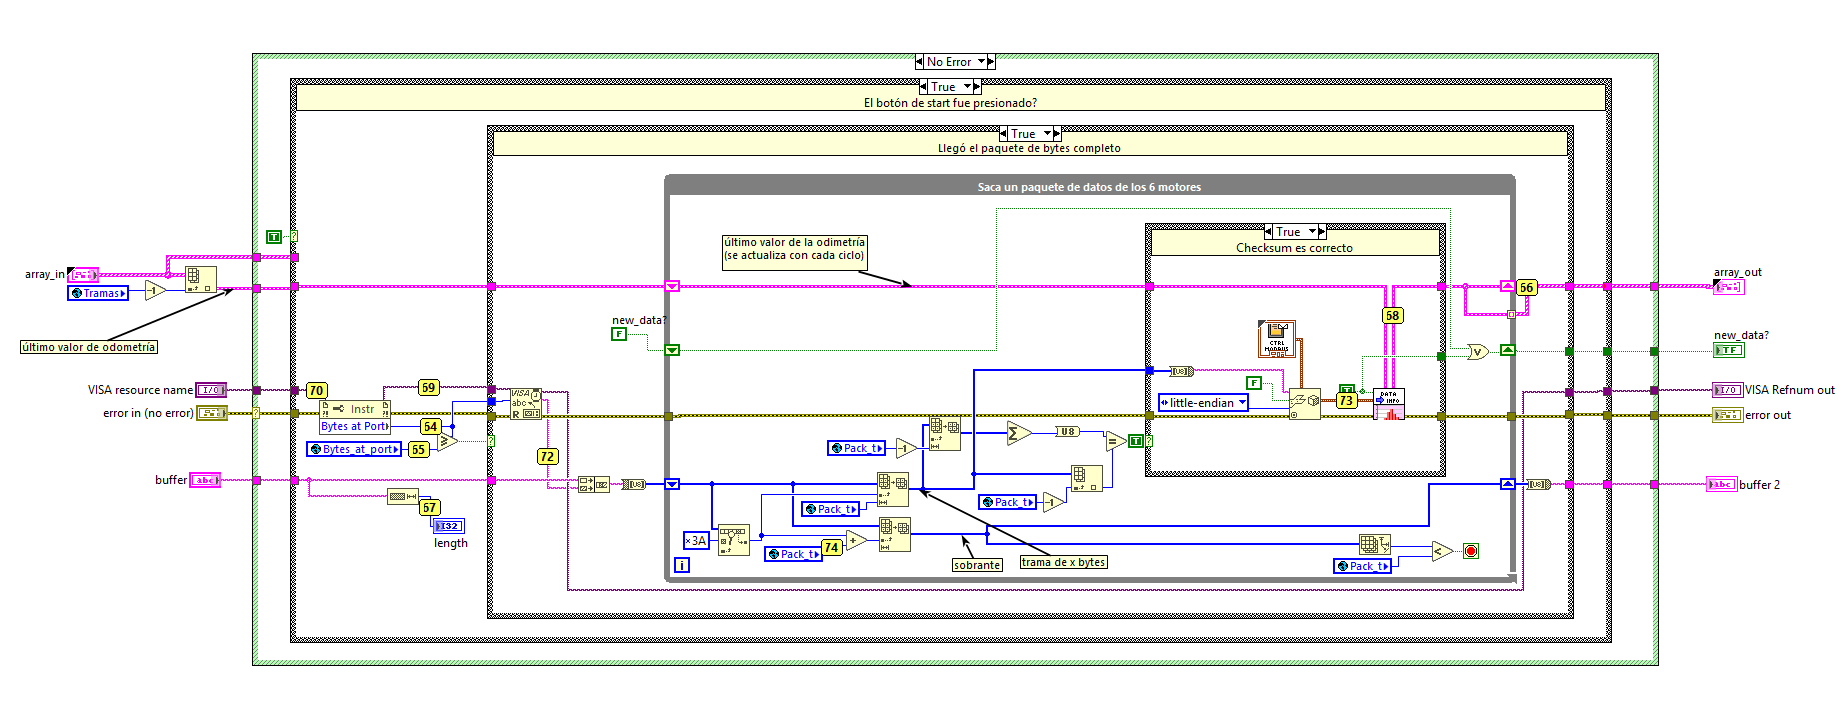
\includegraphics[width=1\linewidth]{images/Interfaz/loopdecodemodbus}
	\caption{Loop del VI de decodeModbusMessage.}
	\label{fig:loopdecodemodbus}
\end{figure}

\clearpage
\subsection{Global init}
Para garantizar el determinismo en la comunicación y la sincronización de los procesos, se implementó un módulo de inicialización global. Este componente define las constantes críticas que el software utiliza para gestionar la telemetría bajo un protocolo inspirado en Modbus, así como la configuración del recurso VISA.

\subsubsection{Variables de Protocolo y Sincronización (MODBUS)}
En esta sección se definen las dimensiones de los paquetes de datos que circulan entre el hardware y el software:

\begin{itemize}
	\item \textbf{T\_muestreo (0.004):} Define el intervalo de tiempo (4 ms) en el que el Arduino realiza el muestreo de los pasos del encoder. Esta constante es fundamental para el cálculo preciso de la velocidad en el Dashboard.
	\item \textbf{Pack\_t (31):} Especifica el tamaño fijo de cada \textbf{Trama} individual (31 bytes). Este valor debe coincidir exactamente con la estructura de datos enviada por el microcontrolador para evitar desfases en la decodificación.
	\item \textbf{Tramas (15):} Indica la cantidad de paquetes que se desean leer en una única iteración del programa.
	\item \textbf{Bytes\_at\_port:} Es una variable calculada dinámicamente (\textit{Pack\_t} $\times$ \textit{Tramas}) que representa el tamaño total del \textbf{Lote de Datos} que el sistema espera encontrar en el búfer serial antes de proceder con el des-empaquetado.
\end{itemize}

\subsubsection{Configuración del Recurso Serial (VISA)}
Parámetros encargados de la robustez de la capa física de comunicación:

\begin{itemize}
	\item \textbf{V\_buf\_t (10000):} Define el tamaño del búfer de memoria asignado a la sesión VISA, permitiendo almacenar ráfagas de datos sin pérdida de información.
	\item \textbf{V\_timeout (100):} Establece el tiempo máximo de espera (100 ms) antes de que la computadora arroje un error de comunicación si el hardware no responde.
	\item \textbf{V\_baud (500000):} Determina la velocidad de transmisión serial. Se ha seleccionado un baudrate elevado para soportar el flujo de telemetría de alta frecuencia requerido por el control PID.
\end{itemize}

\subsubsection{Monitoreo de Estado y Errores}
Adicionalmente, el sistema mantiene contadores de diagnóstico para supervisar la salud del enlace:
\begin{itemize}
	\item \textbf{Contador Correcto/Incorrecto:} Registra la cantidad de tramas que superaron o fallaron la validación del CRC.
	\item \textbf{Estado\_Conexion:} Un indicador booleano global que informa a todos los subpaneles si el enlace con el brazo robótico está activo y listo para operar.
\end{itemize}

\begin{figure}[h]
	\centering
	
\includegraphics[width=0.5\linewidth]{images/Interfaz/globaliniticon}
	\caption{Símbolo del global init.}
	\label{fig:globaliniticon}
\end{figure}

\begin{figure}[h]
	\centering
	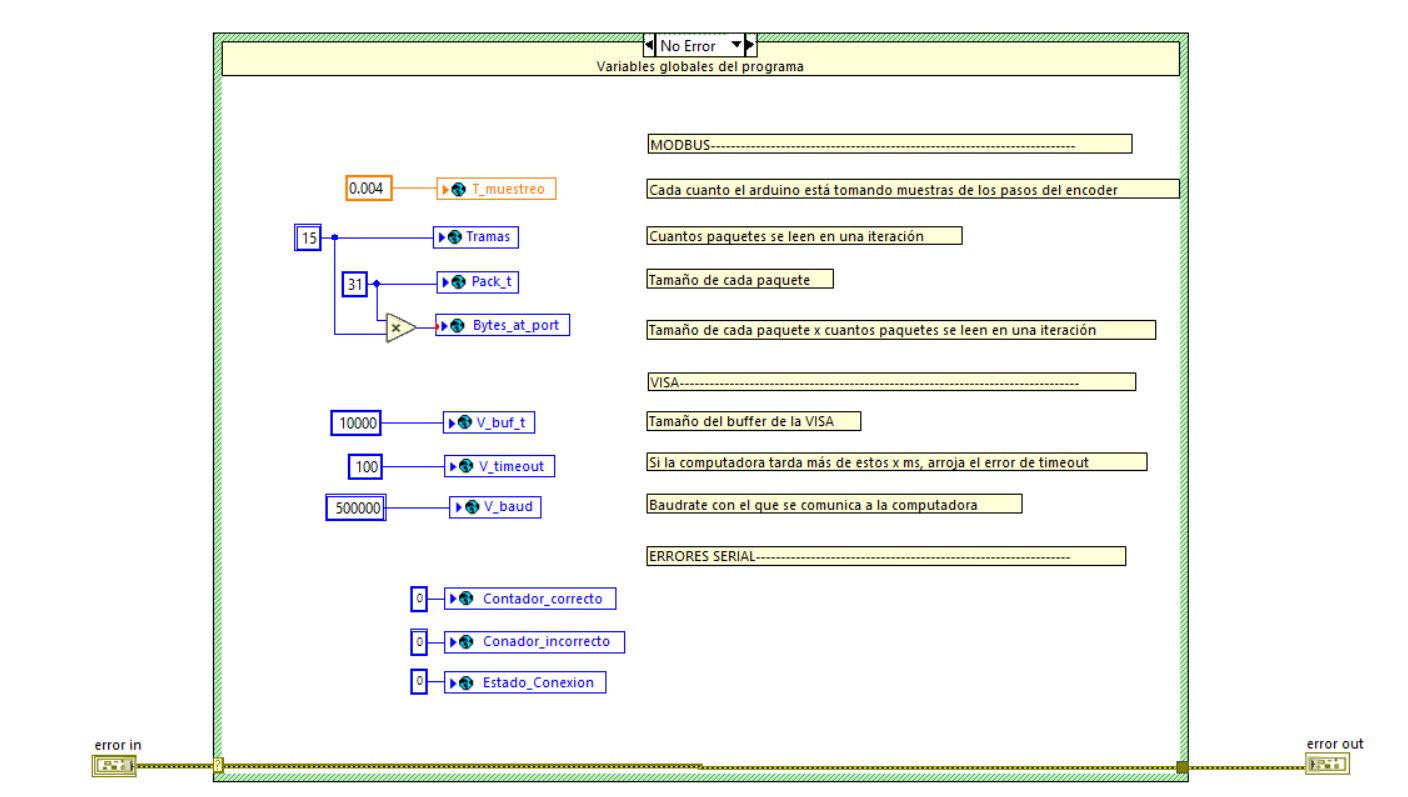
\includegraphics[width=1\linewidth]{images/Interfaz/globaklinit}
	\caption{Al inicio del programa se asignan valores a estas variables. Se creó este VI para centralizar en un lugar la información que puede cambiar el comportamiento del programa y permite hacer cambios fácilmente.}
	\label{fig:globaklinit}
\end{figure}


\clearpage
\begin{resultadosFase}
	\begin{itemize}
		\item \textbf{Latencia Nula:} Gracias al procesamiento por \textit{Lotes de Datos}, la interfaz no presenta retardos ni congelamientos, asegurando una visualización fluida de la telemetría.
		\item \textbf{Integridad de Datos:} El uso del protocolo inspirado en Modbus con validación CRC garantiza la eliminación de ráfagas de ruido y asegura que solo comandos válidos lleguen a los actuadores.
		\item \textbf{Robustez Concurrente:} La implementación de la FGV VISA Write permite el acceso simultáneo de múltiples lazos de control al puerto serial sin generar colisiones ni errores de recurso.
		\item \textbf{Infraestructura Cinemática:} El sistema deja establecida la base de software necesaria (lectura de encoders y envío de tramas PWM/Tiempo) para la futura ejecución de algoritmos de cinemática directa e inversa.
	\end{itemize}
\end{resultadosFase}